%!TEX TS-program = xelatex

% Шаблон документа LaTeX создан в 2018 году
% Алексеем Подчезерцевым
% В качестве исходных использованы шаблоны
% 	Данилом Фёдоровых (danil@fedorovykh.ru) 
%		https://www.writelatex.com/coursera/latex/5.2.2
%	LaTeX-шаблон для русской кандидатской диссертации и её автореферата.
%		https://github.com/AndreyAkinshin/Russian-Phd-LaTeX-Dissertation-Template

\documentclass[a4paper,14pt]{article}


%%% Работа с русским языком
\usepackage[english,russian]{babel}   %% загружает пакет многоязыковой вёрстки
\usepackage{fontspec}      %% подготавливает загрузку шрифтов Open Type, True Type и др.
\defaultfontfeatures{Ligatures={TeX},Renderer=Basic}  %% свойства шрифтов по умолчанию
\setmainfont[Ligatures={TeX,Historic}]{Times New Roman} %% задаёт основной шрифт документа
\setsansfont{Comic Sans MS}                    %% задаёт шрифт без засечек
\setmonofont{Courier New}
\usepackage{indentfirst}
\frenchspacing

\renewcommand{\epsilon}{\ensuremath{\varepsilon}}
\renewcommand{\phi}{\ensuremath{\varphi}}
\renewcommand{\kappa}{\ensuremath{\varkappa}}
\renewcommand{\le}{\ensuremath{\leqslant}}
\renewcommand{\leq}{\ensuremath{\leqslant}}
\renewcommand{\ge}{\ensuremath{\geqslant}}
\renewcommand{\geq}{\ensuremath{\geqslant}}
\renewcommand{\emptyset}{\varnothing}

%%% Дополнительная работа с математикой
\usepackage{amsmath,amsfonts,amssymb,amsthm,mathtools} % AMS
\usepackage{icomma} % "Умная" запятая: $0,2$ --- число, $0, 2$ --- перечисление

%% Номера формул
%\mathtoolsset{showonlyrefs=true} % Показывать номера только у тех формул, на которые есть \eqref{} в тексте.
%\usepackage{leqno} % Нумерация формул слева	

%% Перенос знаков в формулах (по Львовскому)
\newcommand*{\hm}[1]{#1\nobreak\discretionary{}
	{\hbox{$\mathsurround=0pt #1$}}{}}

%%% Работа с картинками
\usepackage{graphicx}  % Для вставки рисунков
\graphicspath{{images/}}  % папки с картинками
\setlength\fboxsep{3pt} % Отступ рамки \fbox{} от рисунка
\setlength\fboxrule{1pt} % Толщина линий рамки \fbox{}
\usepackage{wrapfig} % Обтекание рисунков текстом

%%% Работа с таблицами
\usepackage{array,tabularx,tabulary,booktabs} % Дополнительная работа с таблицами
\usepackage{longtable}  % Длинные таблицы
\usepackage{multirow} % Слияние строк в таблице
\usepackage{float}% http://ctan.org/pkg/float

%%% Программирование
\usepackage{etoolbox} % логические операторы


%%% Страница
\usepackage{extsizes} % Возможность сделать 14-й шрифт
\usepackage{geometry} % Простой способ задавать поля
\geometry{top=20mm}
\geometry{bottom=20mm}
\geometry{left=20mm}
\geometry{right=10mm}
%
%\usepackage{fancyhdr} % Колонтитулы
% 	\pagestyle{fancy}
%\renewcommand{\headrulewidth}{0pt}  % Толщина линейки, отчеркивающей верхний колонтитул
% 	\lfoot{Нижний левый}
% 	\rfoot{Нижний правый}
% 	\rhead{Верхний правый}
% 	\chead{Верхний в центре}
% 	\lhead{Верхний левый}
%	\cfoot{Нижний в центре} % По умолчанию здесь номер страницы

\usepackage{setspace} % Интерлиньяж
\onehalfspacing % Интерлиньяж 1.5
%\doublespacing % Интерлиньяж 2
%\singlespacing % Интерлиньяж 1

\usepackage{lastpage} % Узнать, сколько всего страниц в документе.

\usepackage{soul} % Модификаторы начертания

\usepackage{hyperref}
\usepackage[usenames,dvipsnames,svgnames,table,rgb]{xcolor}
\hypersetup{				% Гиперссылки
	unicode=true,           % русские буквы в раздела PDF
	pdftitle={Разработка программной системы для автоматической генерации графа диалогов по текстам пьес.},   % Заголовок
	pdfauthor={Подчезерцев А.Е.},      % Автор
	pdfsubject={ВКР},      % Тема
	pdfcreator={Подчезерцев А.Е.}, % Создатель
	pdfproducer={Подчезерцев А.Е.}, % Производитель
	pdfkeywords={keyword1} {key2} {key3}, % Ключевые слова
	colorlinks=true,       	% false: ссылки в рамках; true: цветные ссылки
	linkcolor=black,          % внутренние ссылки
	citecolor=black,        % на библиографию
	filecolor=magenta,      % на файлы
	urlcolor=black           % на URL
}
\makeatletter 
\def\@biblabel#1{#1. } 
\makeatother
\usepackage{cite} % Работа с библиографией
%\usepackage[superscript]{cite} % Ссылки в верхних индексах
%\usepackage[nocompress]{cite} % 
\usepackage{csquotes} % Еще инструменты для ссылок

\usepackage{multicol} % Несколько колонок

\usepackage{tikz} % Работа с графикой
\usepackage{pgfplots}
\usepackage{pgfplotstable}

\usepackage{ dsfont }

\newcommand{\imref}[1]{рис.~\ref{#1}}

\usepackage{spreadtab}
\newcolumntype{K}[1]{@{}>{\centering\arraybackslash}p{#1cm}@{}}


\usepackage{xparse}
\usepackage{fancyvrb}

\RecustomVerbatimCommand{\VerbatimInput}{VerbatimInput}
{
	fontsize=\footnotesize    
}

\newcolumntype{?}[1]{!{\vrule width #1}}

\usepackage{tocloft}
\renewcommand{\cftsecleader}{\cftdotfill{\cftdotsep}}

\usepackage{pdfpages}

\usepackage{rotating}

\usepackage{pdflscape}

\usepackage{ragged2e}
\usepackage{microtype}

% Выравнивание по ширине без переносов слов
\justifying
\sloppy
\tolerance=500
\hyphenpenalty=10000
\emergencystretch=3em

% Подогнать таблицу под ширину страницы
\usepackage{adjustbox}

\usepackage{titlesec}

% ГОСТ заголовки таблицы
\usepackage[font=small]{caption}

\captionsetup[figure]{justification=centering,labelsep=period} % Картинки по центру, с точкой после рис

\DeclareCaptionLabelFormat{rightline}{\rightline{\bothIfFirst{#1}{ }#2}}
\captionsetup[table]{justification=centering,labelformat=rightline,labelsep=newline}

\newcommand{\tablecaption}[1]{\addtocounter{table}{1}\small \begin{flushright}\tablename \ \thetable\end{flushright}%	
	\begin{center}#1\end{center}}

\usepackage{enumerate}
\begin{document} % конец преамбулы, начало документа
	 \begin{titlepage}
	\begin{center}
 		ФЕДЕРАЛЬНОЕ  ГОСУДАРСТВЕННОЕ АВТОНОМНОЕ \\
		ОБРАЗОВАТЕЛЬНОЕ УЧРЕЖДЕНИЕ ВЫСШЕГО ОБРАЗОВАНИЯ\\
		«НАЦИОНАЛЬНЫЙ ИССЛЕДОВАТЕЛЬСКИЙ УНИВЕРСИТЕТ\\
		«ВЫСШАЯ ШКОЛА ЭКОНОМИКИ»
	\end{center}
	
	\begin{center}
		\textbf{Московский институт электроники и математики}
		
		\textbf{им. А.Н.Тихонова НИУ ВШЭ}
		
		\vspace{2ex}
		
		\textbf{Департамент компьютерной инженерии}
	\end{center}
	\vspace{1ex}	
	
	\begin{center}
		Курс «Системное проектирование цифровых устройств»
	\end{center}	
	
	
	\begin{center}
	\textbf{ОТЧЕТ\\
		ПО ЛАБОРАТОРНОЙ РАБОТЕ №1
	}
	\end{center}	

	\begin{center}
		Тема работы: «Разработка и программирование Soft-процессорных ядер с архитектурой однотактный MIPS. Часть 1»
	\end{center}

	\vspace{2ex}

	\begin{flushright}
		\textbf{Выполнили:}
		
		\vspace{2ex}
		
		Студенты группы БИВ174
		
		Бригада №5
		
		\vspace{2ex}
		
		Подчезерцев Алексей Евгеньевич
		
		Солодянкин Андрей Александрович
		\vspace{2ex}
		
		\textbf{Принял:}
		
		асс. МИЭМ НИУ ВШЭ
		
		Американов А.А.
		
	\end{flushright}

	\vfill
	\begin{center}
		Москва \the\year \, г.
	\end{center}
	
\end{titlepage}
\addtocounter{page}{1}
	
	\tableofcontents
	
	\pagebreak
	%\section{Индивидуальное задание}
	
	%\pagebreak
	
	%-
	
	%\pagebreak
	
	%\section{Дневник практики}
	
	%\pagebreak
	
	%-
	
	%\pagebreak
	
	
	\section{Введение}
	
	Целью данной практики является закрепление и развитие профессиональных компетенций научно-исследовательской и проектной деятельности.
	Для достижения поставленной цели потребовалось решить следующие задачи практики (в соответствии с программой практики):
	
	\begin{itemize}
	
		\item Закрепление и расширение теоретических и практических знаний, полученных студентом в процессе обучения;
		
		\item Получение навыков самостоятельной работы, а также работы в составе научно-исследовательских коллективов.
		
		\item Работа над исследованием по анализу аффинных преобразований в семантическом пространстве BERT.
		
		\item Обработка полученных материалов и оформление отчета о прохождении практики.
			
	\end{itemize}

	Исследование проводится на языке python в среде Jupyter Notebok при использовании Google Colab. Jupyter Notebok является наиболее удобной платформой для проведения исследований на python.
	Google Colab является бесплатной и мощной платформой для запуска кода.
	При этом дается 12Гб оперативной памяти, доступ к Google диску для доступа к данным, а также есть возможность запускать код с использованием GPU.
	
	\pagebreak
	\section{Содержательная часть}
	
	\subsection{Описание профессиональных задач студента}
	
	%Целью данной работы является исследование и измерение качества аффинных преобразований для модели BERT.
	
	Для проведения исследования по анализу аффинных преобразований в семантическом пространстве BERT необходимо решить следующие задачи:
	
	\begin{itemize}
		
		\item Исследование моделей векторного представления слов;
		
		\item Исследование методов оценки аффинных преобразований;
		
		%\item Постановка задачи пропорциональной аналогии в терминах аффинного преобразования;
		
		\item Разработка метода оценки точности параллельного переноса для контекстуализированных моделей;
		
		\item Подготовка экспериментальных данных;
		
		\item Проведение экспериментов;
		
		\item Оценка полученных результатов.
		
	\end{itemize}
	
	
	\subsection{Исследование моделей векторного представления слов}
	
	Векторное представление слов — метод обработки естественного языка, в основе которого лежит идея представить каждое слово или токен в виде вектора определенной размерности.
	
	\subsubsection{One-hot encoding}
	
	Самой простой реализацией модели векторного представления слов является one-hot encoding.
	Идея этой модели заключается в том, что в наборе из $K$ слов каждому слову соответствует вектор длиной $K$ со всеми нулями и единицей с позицией $i$, где $i$ - это номер слова во всем наборе.
	Недостатком этого метода является то, что по данным векторным представлениям нельзя судить о схожести слов.
	Также для больших наборов слов размер векторных представлений будет очень большим, из-за чего их неэффективно хранить в памяти.
	
	\subsubsection{Word2vec}
	
	Word2vec одна из первых моделей, использующих нейронные сети для создания векторных представлений слов.
	Идея создания векторов в word2vec основана на предположении о контекстной близости, а именно на том, что слова встречающиеся в одинаковых контекстах скорее всего имеют схожее значение.
	Предлагается проверять схожесть слов при помощи косинусного сходства их векторных представлений (\ref{eq:cos_sim}).
	
	\begin{equation}
		similarity(A,B) = cos(A,B) = cos(\theta) = \dfrac{A\cdot B}{\|A\| \|B\|}
		\label{eq:cos_sim}
	\end{equation}

	где
	
	$A$ - векторное представление первого слова,
	
	$B$ - векторное представление второго слова,
	
	$\theta$ - угол между векторами $A$ и $B$.
	
	Существует 2 метода обучения word2vec: kip-gram и CBOW (Continuous Bag of Words).
	В Skip-gram по слову прогнозируется слова из его контекста, в CBOW, наоборот, по контексту предсказывается слово.
	В качестве выходного слоя в моделях применяется функция softmax в различных вариациях для того.
		
	\subsubsection{FastText}
	
	FastText является продолжением развития модели word2vec.
	При этом в fastText отличается от word2vec тем, что у новой модели используются N-граммы символов.
	Например, для слова молоко 3-граммами являются мол, оло, лок, око.
	Векторные представления строятся именно для N-грамм, векторные представления слов - это сумма векторных представлений всех его N-грамм.
	При этом решается проблема того, что словарь модели word2vec был ограничен.
	Использование N-грамм позволяет получать векторные представления для редких слов.
	
	\subsubsection{ELMO}
	
	ELMO была одной из первых моделей обработки естественного языка, которая учитывала контекст слова.
	Для моделей word2vec или fastText при вычислении векторного представления не учитывается контекст слова, для омонимов и омографов представления будут одинковыми.
	В ELMO решается эта проблема, в основе этой модели лежит многослойная двунаправленная рекуррентная нейронная сеть c LSTM (Long short-term memory).
	
	\subsubsection{BERT}
	
	Модель BERT или Bidirectional Encoder Representations from Transformers была опубликована командой Google AI в 2018 году.
	На момент появления модель BERT показала лучшее качество на тесте SQuAD 1.1.
	
	BERT состоит из 12 следующих друг за другом энкодеров.
	Каждый энкодер состоит из компонентов, первый компонент - это слой внутреннего внимания (self-attention), второй - нейронная сеть прямого распространения (feed-forward neural network).
	
	Обучение модели BERT основывается на следующих принципах.	
	Первый основывается на том, чтобы заменить 15\% слов масками и обучить модель предсказывать эти слова.
	Этот принцип позволяет модели самой обучаться на полноценных текстах без предварительной разметки, что позволило обучить BERT на огромном массиве данных.
	Вторая идея состоит в том, чтобы дополнительно научить BERT определять, является ли одно предложение логичным продолжением другого.
	
	\subsection{Исследование методов оценки аффинных преобразований}
	
	В основе большинства методов оценки аффинных преобразований лежит описанное в формуле (\ref{eq:cos_sim}) косинусное сходство.
	Для удобства применяется также косинусное расстояние (\ref{eq:cos_dist}).
	
	\begin{equation}
		distance(A,B) = 1 - similarity(A,B)
		\label{eq:cos_dist}
	\end{equation}

	Аффинные преобразования над векторными представлениями слов предполагают задачу пропорциональной аналогии.
	Задача пропорциональной аналогии заключается в том, чтобы установить для группы пар слов определенную логическую связь в парах.
	Рассмотрим группу пар слов $(a: a^*), (b: b^*)$. 
	Известно, что слова в первой группе относятся друг к другу также, как и слова во второй группе.
	Представить это можно следующим образом (\ref{eq:preobr}).
	
	\begin{equation}
		(a: a^*) :: (b: b^*)
		\label{eq:preobr}
	\end{equation}

	Если в парах действует одна и та же связь, то можно выразить одно из слов через 3 других слова (\ref{eq:yravn}).
	
	\begin{equation}
		y = v_b - v_a + v_{a^*}
		\label{eq:yravn}
	\end{equation}
	 
	 где 
	 
	 $y$ - искомый вектор,
	 
	 $v_x$ - эмбеддинг для слова $x$.
	 
	 Но вектору $y$ может не соответствовать ни одного слова, поэтому в качестве ответа берется ближайшее слово к $y$.
	 Для корректно работающей модели ответ совпадет с $b^*$.
	 Результат можно выразить формулой (\ref{eq:3cosadd}).
	 
	 \begin{equation}
	 	y^* = \underset{v \notin \{v_b, v_a, v_{a^*}\}}{argmax} \; cos(v, v_b - v_a + v_{a^*})
	 	\label{eq:3cosadd}
	 \end{equation}
	 
	 
	%Возникает необходимость оценить в качество решения задачи пропорциональной аналогии.
	Интуитивно понятным способом оценить качество будет сопоставить все пары слов друг с другом, посчитать одно из слов по формуле (\ref{eq:3cosadd}) и найти среднее значение косинусной близости после трансформаций.
	Данный способ получил название \textbf{3CosAdd}.
	
	Существует пердположение, что \ref{eq:3CosMul} эквивалентно (\ref{eq:3cosadd}). Этот метод получил название \textbf{3CosMul}.
	
	\begin{equation}
		y^* = \underset{v \notin \{v_b, v_a, v_{a^*}\}}{argmax} \; cos(v, v_{a^*}) - cos(v, v_a) + cos(v, v_b)
		\label{eq:3CosMul}
	\end{equation}

	Если в группе у пар одна и та же связь, то можно посчитать среднюю разницу между векторами в парах и задача аналогии будет решаться через посчитанную разницу.
	Эта идея предлагается в метрике	\textbf{3CosAvg} (\ref{eq:3CosAvg}).
	
	\begin{equation}
		y^* = \underset{v \notin \{v_b, v_a, v_{a^*}\}}{argmax} \; cos(v,v_b + \dfrac{\sum_{i=1}^{n}v_{a_i^*}}{n} - \dfrac{\sum_{i=1}^{n}v_{a_i}}{n})
		\label{eq:3CosAvg}
	\end{equation}
	
	Существуют и другие методы оценки аффинных преобразований.
	Метод \textbf{Only-b} основан на предположении, что вектора $v_b$ и $v_{b^*}$ находятся максимально близко друг к другу (\ref{eq:Only-b}).
	
	\begin{equation}
		y^* = \underset{v \notin \{v_b, v_a, v_{a^*}\}}{argmax} \; cos(v, v_b)
		\label{eq:Only-b}
	\end{equation}

	В методе \textbf{Ignore-a} предполагается, что результат ближе всего к сумме векторов $v_b$ и $v_{a^*}$ (\ref{eq:Ignore-a}).
	
	\begin{equation}
		y^* = \underset{v \notin \{v_b, v_a, v_{a^*}\}}{argmax} \; cos(v, v_b + v_{a^*})
		\label{eq:Ignore-a}
	\end{equation}

	В методе \textbf{Add-opposite} результатом является вектор, ближайший к выражению $-(v_{a^*} - v_a) + v_b$ (\ref{eq:Add-opposite}).

	\begin{equation}
		y^* = \underset{v \notin \{v_b, v_a, v_{a^*}\}}{argmax} \; cos(v, -(v_{a^*} - v_a) + v_b)
		\label{eq:Add-opposite}
	\end{equation}

	Метод \textbf{MULTIPLY} имеет следующий вид (\ref{eq:MULTIPLY}).
	
	\begin{equation}
		y^* = \underset{v \notin \{v_b, v_a, v_{a^*}\}}{argmax} \; \dfrac{cos(v, v_{a^*}) \; cos(v, v_b)}{cos(v, v_a)}
		\label{eq:MULTIPLY}
	\end{equation}
	
%	\subsection{Постановка задачи пропорциональной аналогии в терминах аффинного преобразования}
%	3
	
	\subsection{Разработка метода оценки точности параллельного переноса для контекстуализированных моделей}
	
	Для контекстуализированных моделей описанные ранее методы в чистом виде не применимы.
	Для одних и тех же слов в разных контекстах будут получаться разные эмбеддинги.
	Получить единственный эмбеддинг для токена можно после усреднения всех полученных эмбеддингов для этого токена.
	В результате каждому токену будет соответствовать только одно векторное представление.
	
	После получения усредненных эмбеддингов для всех токенов можно применять описанные ранее методы оценки аффинных преобразований.
	
	\subsection{Подготовка экспериментальных данных}
	
	Для получения эмбеддингов слов были взяты тексты из электронной библиотеки КиберЛенинка.
	Тексты двух жанров: литература и политика.
	
	Для оценки качества аффинных преобразований используется датасет $Google\_analogy\_test\_set$.
	Данный датасет был переведен на русский язык с сохранением семантических отношений между словами.
	Не все слова из данного датасета есть в словаре BERT, поэтому часть отношений пришлось убрать.
	
	\subsection{Проведение экспериментов}
	
	Для проведения экспериментов используется язык программирования python в среде Jupyter Notebok с использованием Google Colab.
	Jupyter Notebok является наиболее удобной платформой для проведения исследований на python.
	Google Colab является бесплатной и мощной платформой для запуска кода.
	При этом дается 12Гб оперативной памяти, доступ к Google диску для доступа к данным, а также есть возможность запускать код с использованием GPU.
	В качестве фреймворка для работы с моделью BERT был выбран pytorch, так как это современная и гибкая библиотека для работы с глубинным обучением.
	
	Для проведения экспериментов необходимо подготовить данные для их обработки в модели BERT.
	Сначала весь текст разбивается на отдельные предложения, далее происходит их токенизация и индексация.
	На этом этапе обработанные предложения по-одному отправляются в модель BERT.
	Данным способом обработаны по 1 миллиону предложений для каждого жанра.
	
	Полученные после обработки объекты представляют из себя четырёхразмерные тензоры, где оси отражают следующую информацию (в скобках представлено количество элементов):
	
	\begin{enumerate}
		
		\item Номер слоя (13 слоев);
		
		\item Номер батча (1 предложение);
		
		\item Количество слов/токенов в предложении (количество токенов в предложении);
		
		\item Векторное представление (768 свойств).

	\end{enumerate}	

	По оси слоев первый слой - это эмбеддинг, поступающий на вход модели, остальные 12 слоев отображают выходы 12 энкодеров.
	Номер батча в нашем случае не важен, так как используется только одно предложение.
	Следующая ось отображает токены в предложении с сохранением порядка.
	Последняя ось отвечает за векторное представление каждого токена.
	
	Получить итоговое векторное представление для токена можно несколькими способами (рисунок \ref{fig:dif_vars_get_v}).
	В нашем случае используется способ с суммированием последних четырех слоев, данный способ показывает хорошее качество.
	Способ с конкатенацией последних четырех не используется, так как он требует в 4 раза больше ресурсов.
	
	Описанным ранее методом обрабатываются все подготовленные предложения.
	Обработка происходит пачками по 10 тысяч предложений.
	Векторные представления токенов каждой пачки сохраняются на Google диск.
	Сделано это из-за ограничений оперативной памяти устройства.
	
	После того как получены векторные представления для всего текста, считаются средние эмбеддинги для всех токенов.
	Из-за ограничений оперативной памяти нельзя посчитать сразу все векторные представления, поэтому они считаются порциями с сохранением промежуточных результатов.
	
	Далее проверялось семантические отношения полученных эмбеддингов на переведенном датасете $Google\_analogy\_test\_set$.
	В качестве метрик были взяты 3CosAdd, 3CosAvg и 3CosMul.
	
	\subsection{Оценка полученных результатов}
	
	На рисунках \ref{fig:liter} и \ref{fig:politics} представлены результаты аффинных преобразований для литературы и политики соответственно.
	
	Первая колонка type описывает вид связи в группе.
	Строка metric указывает использованную метрику.
	Колонка result отражает долю верных ответов.
	Колонка cosine отображает среднее косинусное расстояние между посчитанным эмбеддингом и правильным эмбеддингом.
	Последнняя колонка описывает количество тестов в группе.
	
	Данные результаты показывают, что аффинные преобразования в модели BERT возможны, но их качество плохое.
	Это может быть связано с тем, что в эмбеддингах помимо семантического смысла может скрываться какая-то другая информация о словах.
	Еще одной из возможных причин плохого качества может быть то, что исследование проводилось на русском языке и не все слова из тестового датасета были в словаре модели BERT.
	
	
	\pagebreak
	\section{Заключение}
	
	В ходе практики, были изучены модели векторного представления слов, рассмотрены самые популярные архитектуры моделей преобразования слов в эмбеддиги.
	
	Были приобретены навыки по поиску необходимого датасета, по работе и применению модели BERT.
	%Помимо этого, были получены навыки по работе с графическим интерфейсом в python.
	
	По окончанию практики была достигнута главная цель - применение теоретических знаний, полученных в процессе обучения, в реальной экспериментальной задаче.
	
	А также приобретены навыки и опыт практической работы с NLP.
	Данная практика является хорошим практическим опытом для дальнейшей самостоятельной деятельности.
	
	\pagebreak
	\section{Приложения}
	
	С кодом можно ознакомиться по ссылке:

 \href{https://github.com/andrsolo21/hse_Af_Tr_BERTn}{https://github.com/andrsolo21/hse\_Af\_Tr\_BERT}.
	

	
\begin{figure}[H]
	\centering
	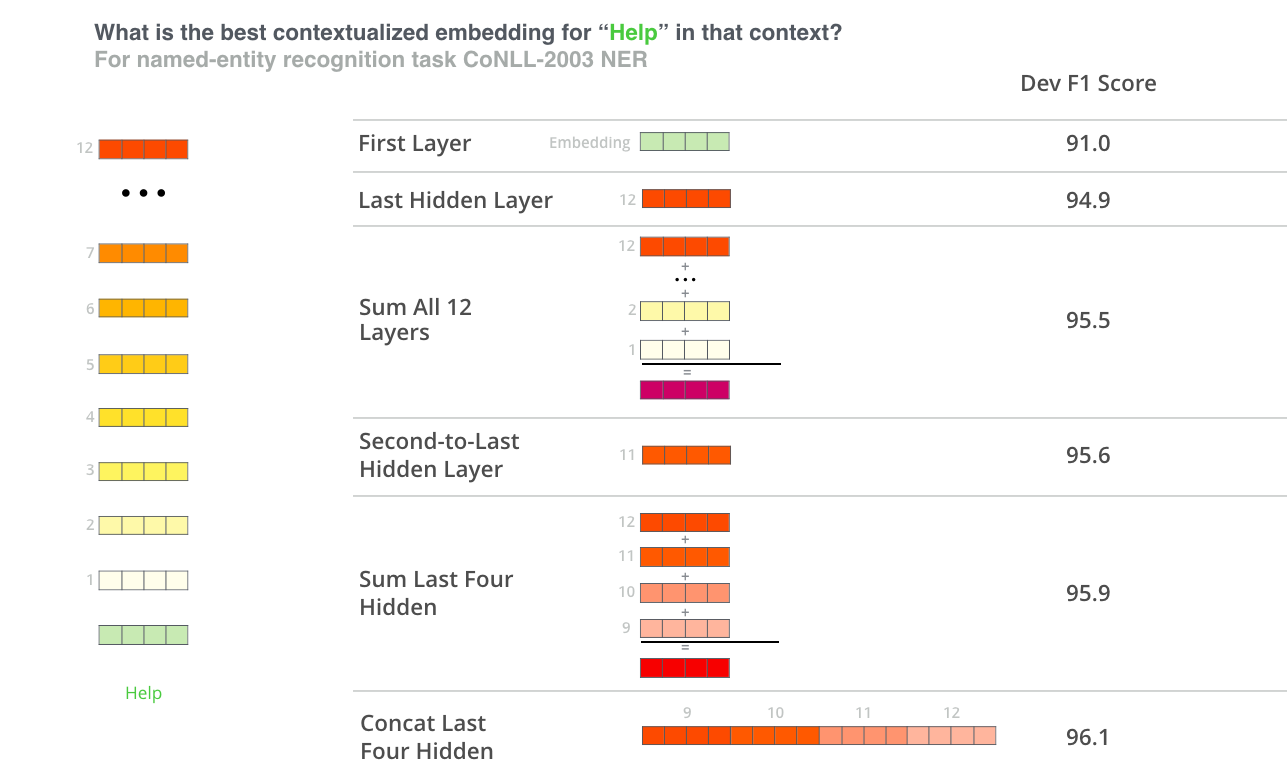
\includegraphics[width=0.7\linewidth]{image/irvrsv9mefroz7io6ilnjng3fo4}
	\caption{Возможные варианты получения векторного представления}
	\label{fig:dif_vars_get_v}
\end{figure}

\begin{figure}[H]
	\centering
	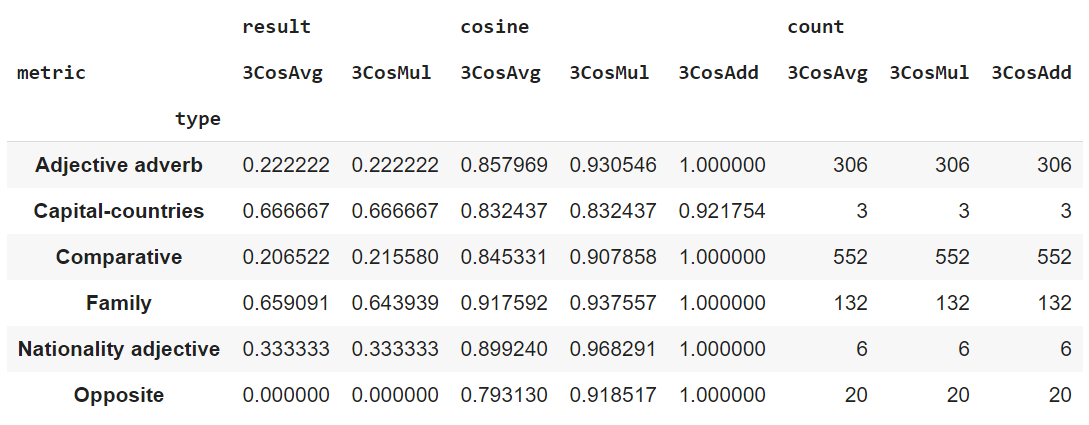
\includegraphics[width=0.7\linewidth]{image/liter}
	\caption{Результаты тестирования для текста с литературой}
	\label{fig:liter}
\end{figure}

\begin{figure}[H]
	\centering
	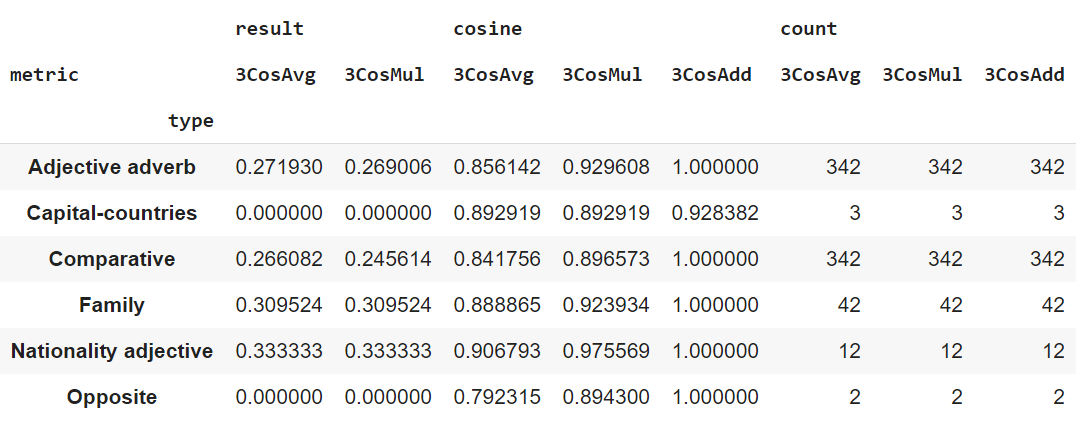
\includegraphics[width=0.7\linewidth]{image/politics}
	\caption{Результаты тестирования для текста с политикой}
	\label{fig:politics}
\end{figure}


	%\newpage 
	%\renewcommand{\refname}{{\normalsize Список использованных источников}} 
	%\centering 
	%\begin{thebibliography}{9} 
	%	\addcontentsline{toc}{section}{\refname} 
	%	\bibitem{Verilog} Thomas D., Moorby P. The Verilog Hardware Description Language. – Springer Science \& Business Media, 2008.
	%	\bibitem{Quartus} Антонов А., Филиппов А., Золотухо Р. Средства системной отладки САПР Quartus II //Компоненты и технологии. – 2008. – №. 89.
	%\end{thebibliography}
	
\end{document} % конец документа